% File: anss2013-cotterell-medina.tex
% Author: Terrance Medina and Michael Cotterell
%
\documentclass[letterpaper,twocolumn,12pt]{article}
\usepackage[utf8]{inputenc}
\usepackage[english]{babel}
\usepackage{scs}
\usepackage{graphicx}
\usepackage{amsmath,amsfonts,amssymb,amsthm}
\usepackage{epsfig,epstopdf}
\usepackage{hyperref}
\usepackage{tkz-graph}
%\usepackage{citesort}

\usetikzlibrary{arrows}

\renewcommand{\topfraction}{0.95}
\renewcommand{\bottomfraction}{0.95}
\renewcommand{\textfraction}{0.05}
\renewcommand{\floatpagefraction}{0.35}


\begin{document}

\newtheorem{defn}{Definition}

\title{A Markov Model for Ontology Alignment}

\author{Michael E. Cotterell and Terrance Medina \\
Department of Computer Science \\
The University of Georgia \\
Athens, GA 30602-7404 \\
mepcott@uga.edu, medinat@uga.edu
}

\maketitle

\begin{abstract}
Ontology Alignment -- problem importance

Need for a way to determine convergence.

How does a Markov chain perform analytically?

\end{abstract}


\section{Introduction}

\begin{itemize}
\item Normalized Levenshtein Disance~\cite{yujian:2007:levenshtein}. 
\item Similarity Flooding~\cite{melnik:2002:similarity}.
\item Probability and Computing book~\cite{mitzenmacher:2005:probability}.
\item Information-Theoretic~\cite{lin:1998:information}.
\item Hungarian algorithm~\cite{kuhn:1955:hungarian}.
\item Ontology Matching book~\cite{euzenat:2007:ontology}.
\item ScalaTion~\cite{miller:2010:scalation}.
\item BCNN book~\cite{bcnn:2010:simulation}.
\item Scala spec~\cite{odersky:2011:spec}.
\end{itemize}

%Knowledge bases
A knowledge base is a kind of database that is designed 
for decision support systems and expert systems. It specifically allows
machines to perform deductive reasoning over its elements.
For example, given the instance data ``John is a farmer'' and ``Farmers
wear overalls'', a knowledge base reasoner could deduce the new information
that ``John wears overalls''.

%KB representation
Knowledge bases (KBs) consist of entities and
relations between those entites. They are often represented as sets of
triples, that is, a set of two entities and a relationship between those
entities. For example, the triple ${\{teachers, lesson\_plans, write\}}$
defines the relationship that teachers write lesson\_plans.

%Ontologies
Ontologies describe the relationships between elements in a knowledge base.
Similar to the notion of schemas in relational databases, ontologies specify
the structural relationships amongst the entities and classes of the ontology.

%Heterogeneous Data Problem
Frequently, queries must be performed across multiple knowledge bases. This is the
case when departments in a large enterprise maintain their own knowledge bases,
but must also share information with other departments. It is also a fundamental
requirement of the semantic web; users perform queries against the web,
and those queries must be performed against knowledge bases that may belong to 
entities on opposite sides of the globe. This leads us to the problem of heterogeneous
data. When knowledge bases are maintained by different organizations, the ontologies
used to describe them will usually be different. They will use different names
to describe similar or identical concepts, for instance, one ontology may keep track
of `cars' while another keeps track of `automobiles' and still another keeps track of 
`autoProducts'. In fact the list could go on and on.

%Ontology Alignnment
Ontology Alignment is the process of equating two heterogeneous ontologies by
finding valid correspondences between their sets of elements. 
%
For instance, an alignment between an auto parts manufacturer and an auto dealership
might tell us with 85\% certainty that ``anti\_lock\_brakes'' and ``ABS'' represent
the same thing.

%Importance of Ontology Alignment
This is important because it allows a query management system to translate the terminology
of a user's query into the terminology used by many different ontologies and thereby
to query heterogeneous knowledge bases.

%Contribution
We present a novel representation for ontology alignment that allows for improved
convergence analysis.

\subsection{Why do we need fully automated alignment?}

\subsection{Background}

%Markov Processes
A Markov Process is a mathematical model that represents a system as a set of states
and a set of probabilistic transitions between those states. Most importantly, Markov 
processes adhere to the Markov Property, that is, a system's next state depends only
on its current state, and not on any of its previous states. In that sense, Markov
processes are called ``memoryless''.

%Hidden Markov Models
A Hidden Markov Model (HMM) is simply a Markov process whose states and transitions
are unobservable.

\section{Related Work}

Although the problem of fully-automated ontology alignment is far from being solved,
there has been much work accomplished around fundamental techniques for element
matching and aggregation of those matching techniques. One class of approaches
attempts to find element matches based on the relative similarity or dissimilarity
of the actual labels giving to those elements. Some examples of these string-matching 
techniques are the Jaro-Winkler measure, the Levenshtein Distance and latent semantic 
indexing.
%
While useful in many situations, string-based matching techniques suffer from a common 
shortcoming; similar real-world objects often have very dissimilar names. The words
``car'' and ``autombile'' provide a good example.

Another class of techniques makes use of outside resources as aids in the search for
good matches between elements. Such outside resources include dictionaries or taxonomies
such as the WordNet taxonomy. These classes of techniques attempt to produce correspondences
between elements that may likely refer to the same real-world objects, but that have very
dissimilar names, such as ``car'' and ``automobile''. Some examples of these semantic 
approaches include Information-theoretic similarity.
%
The use of outside taxonomies can greatly improve the quality of matching results,
but such outside resources are not always readily available.

Yet a third class of matching techniques attempts to exploit the structure of the ontology
itself. For example, Similarity Flooding takes a directed graph representation of an 
ontology and uses neighbor relations between the elements to find matches correspondences
between them. The idea is that if two elements in heterogeneous ontologies are very similar,
then their neighboring elements should also be very similar.
%
%Convergence Properties
Similarity flooding has been useful as a foundation is several other structure-based
matching techniques such as anchor flooding \textbf{**others??*} but suffers from 
a few limitations. First, it requires that the edges of the edge-labeled graph 
representation have identically named labels. It can also be difficult to predict
wether or not the fixpoint calculation will converge.
\newline

\section{Approach}
Testing

\begin{defn}
Let $\gamma$ be some threshold. Edge confidence $\Gamma \left( \alpha, \beta \right)$ is the similarity score between the labels of two edges $\alpha$ and $\beta$ if that similarity is greater than $\gamma$, otherwise $0$. That is,
$$ \Gamma \left( \alpha, \beta \right) = \left\{
   	 \begin{array}{ll}
       \sigma \left( \alpha, \beta \right) & : \vert \sigma \left( \alpha, \beta \right) \vert \geq \gamma \\
       0                                   & : \mathrm{otherwise}
     \end{array}
   \right.$$
\end{defn}

\begin{defn}
Let $x$ and $y$ be terms in a single ontology. The label set $\Lambda \left( x, y \right)$ is the set of all labels between hierarchical properties and object properties where $x$ and $y$ are the domain and range of a property, respectively.
\end{defn}

\begin{figure*}
\centering
\begin{equation*}
\sigma 
\left( \alpha_i, \beta_j \right) = \left\{
	\begin{array}{ll}
   	 	0 &: i=j=0 \\
		i &: j = 0 \text{ and } i > 0 \\
		j &: i = 0 \text{ and } j > 0 \\
		\min 
			\left\{ 
			\begin{array}{l}
				\sigma \left( \alpha_{i-1}, \beta_j \right) + 1 \\
          		\sigma \left( \alpha_i, \beta_{j-1} \right) + 1 \\
          		\sigma \left( \alpha_{i-1}, \beta_{j-1} \right) + [\alpha_i \neq \beta_j]
			\end{array} \right. &: \text{else}
     \end{array}
\right.
\end{equation*}
\caption{Levenshtein Edit Distance}
\end{figure*}

\subsection{Unnormalized Pairwise Markov Chain}
TODO

\begin{figure*}
\centering
\SetVertexNormal[
	Shape = circle,
    % FillColor = orange,
    LineWidth = 1pt
]
\SetUpEdge[
	lw = 1pt,
    color = orange,
    labelcolor = white
]
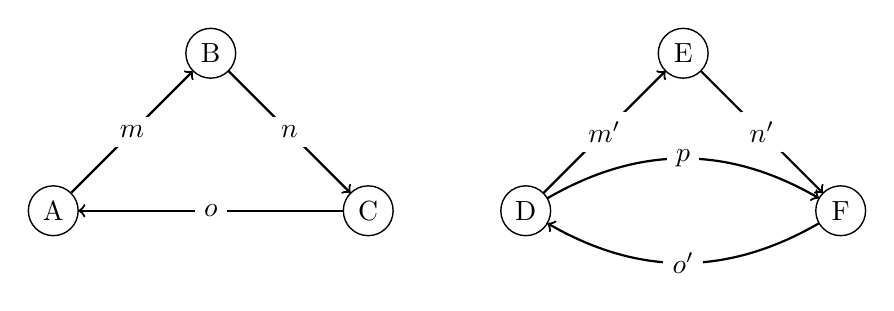
\begin{tikzpicture}
   \Vertex[x=0, y=0]{A}
   \Vertex[x=2, y=2]{B}
   \Vertex[x=4, y=0]{C}
   
   \Vertex[x=6, y=0]{D}
   \Vertex[x=8, y=2]{E}
   \Vertex[x=10, y=0]{F}
%   \tikzset{EdgeStyle/.append style = {bend left}}
   \tikzset{EdgeStyle/.style={->}}
   \Edge[label = $m$](A)(B)
   \Edge[label = $n$](B)(C)
   \Edge[label = $o$](C)(A)
   
   \Edge[label = $m'$](D)(E)
   \Edge[label = $n'$](E)(F)
   \tikzset{EdgeStyle/.append style = {bend left}}
   \Edge[label = $o'$](F)(D)
   \tikzset{EdgeStyle/.append style = {bend left}}
   \Edge[label = $p$](D)(F)  
\end{tikzpicture}
\caption{Example Input Ontologies with Object Properties}
\end{figure*}

\subsection{Normalized Pairwise Markov Chain}
TODO

\section{Evaluation}
TODO

\section{Results}
TODO

\section{Conclusions \& Future Work}
TODO

%ACKNOWLEDGMENTS are optional
\section*{Acknowledgments}
We would like to acknowledge ...

%\bibliographystyle{abbrvnat}
\bibliographystyle{abbrv}
\bibliography{refs} 

\section*{Author Biographies} 
\vspace{8 pt}
\noindent \textbf{MICHAEL E. COTTERELL} is a Ph.D. student in Computer Science at the University of Georgia... His email address is \href{mailto:mepcott@uga.edu}{mepcott@uga.edu}.

\vspace{8 pt}
\noindent \textbf{TERRANCE MEDINA} is a ... His email address is \href{mailto:medinat@uga.edu}{medinat@uga.edu}.




\end{document}


